\chapter{Introduction}

\section{Motivation}
One of the keys factors that has driven transformation of computing industry in the last years is the perception of computing utilities as a commodity\cite{BuYeVeBrBr09}, easily accessible and adjustable to specific needs. As a consequence, we observe a profusion of different services, often collectively referred as a cloud computing \cite{MeGr11}. Similarly to services known from traditional markets, customers expect them to be accessible on demand and in easy manner, while paying only for the consumed goods. Furthermore, customers are interested in a given service only when its provider is eligible to guarantee appropriate quality of service.

The particular service providers that are addressed by this thesis are the ones that supply users with an application execution platform, a model widely known as providing Platform-as-a-Service. In that case, a customer is an entity that has developed an application and is eager to deploy it on an application platform provided that it is able to fulfil his specific requirements, both in terms of quality and cost.

Having customer requirements in mind, it is crucial that a service provider is able to adapt itself to fulfil customer's contract. For example, such adaptation can be triggered by a sudden spike in resource demand and may result in provisioning additional application platforms. However, due to the problem complexity and number of concerns involved, there are different levels where adaptation is possible:
\begin{itemize}
	\item user application
	\item application platform
	\item infrastructure
\end{itemize}
What is more, the fact that a single service provider is constrained by his finite amount of resources poses a risk that it may not be able to serve customer all the time. Consequently, it is expected that adaptation at a service provider level is also possible, i.e. provider can offload some traffic to a different provider, as long as it satisfies a customer.

While self-adaptive systems have a long history \cite{Mu04}, it have not been directly applied to a multi-layered problem that exists in a cloud computing environment. Especially, the research area at the last layer, which sizes across different service providers, is new. Although, architecture known as InterCloud \cite{BuRaCa10} investigates problem of cooperation and negotiation at a cloud level, it neither has been implemented nor presented in a context of self-adaptive system.

\subsection*{Business potential}
The rapid growth of interest in cloud computing in recent years resulted in huge sums of money being invested in the field. Figure \ref{chapter-fig:public-cloud-services-market-size} shows the size of the public cloud services market in 2012 and the forecast of its nearly two times growth in 2016. This data suggests that the subject is attractive for IT industry from the economic point of view. However, higher amounts of money spent on cloud services involve higher expectations of theirs quality from customers. Although the most significant players in cloud computing have been in the field for quite a long time, it is still possible to outline some deficiencies their products have. Additionally, lack of common standards hinder cooperation among different cloud providers. For example it is nearly impossible to create an autoscaling cloud federation with Amazon Web Services (current leader in providing cloud services\cite{GartnerMagicQuadrantSep2013}) and another provider. Amazon EC2, when compared to other companies especially in terms of autoscaling capabilities, really shines. OpenShift, RedHat PaaS solution, ensures application scaling but with very limited possibilities of customisation of the process -- the user can only choose if their application should scale and the whole algorithm is solely based on the number of concurrent requests to the application. Users of Heroku, another PaaS solution, have no automation tool that would control the number of instances (\emph{dynos} in Heroku nomenclature) their application is running on -- they can change it manually.

The proposed solution in this dissertation tries to deal with the aforementioned providers problems by outlining an example architecture that enables seamless cooperation among cloud providers and provides auto-scaling capabilities.

\begin{figure}[!ht]
  \begin{center}
    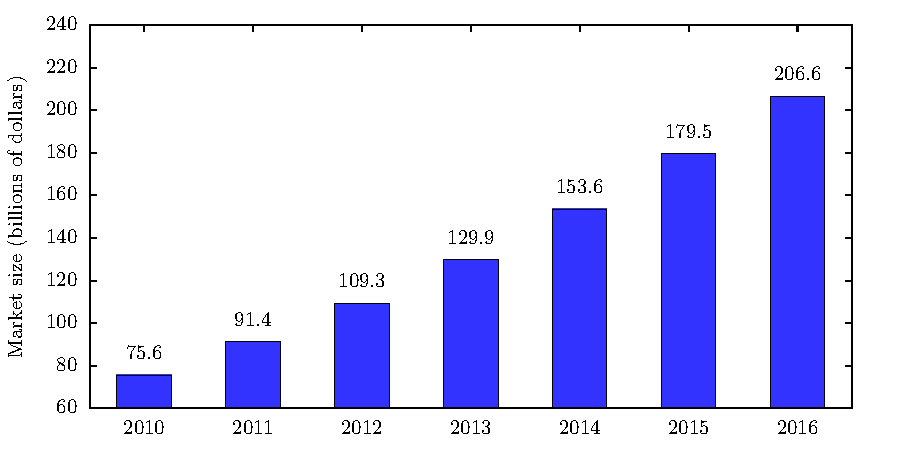
\includegraphics{chapter-introduction/public-cloud-services-market-size}
  \end{center}
  \caption{Public Cloud Services Market Size, 2010-2016 (forecast). Source: \textit{Gartner, 08/2012}}
  \label{chapter-fig:public-cloud-services-market-size}
\end{figure}

\section{Contributions}
The main contributions of this dissertation are as follows:
\begin{itemize}
  \item A proposal of an architecture of a self-adaptive platform that ensures satisfying Quality of Service requirements of deployed users' applications in a cloud computing environment by leveraging horizontal, vertical and cloud-federation-aware scaling
  \item The implementation of the proposed architecture using OpenNebula technology stack
  \item The evaluation of the implemented proof-of-concept solution
\end{itemize}

\section{Impact}
We hope that the concept of self-adaptation at each level of cloud can be thought-provoking for computing scientists.  What is more, we believe that our successful attempt to implement the proposed architecture will cause a greater gain in interest in models that enable scaling applications across different cloud providers, e.g. \emph{InterCloud}.
Finally, we consider the ideas contained in this work be beneficial to the OpenNebula ecosystem as they provide insights into the ways Quality of Service can be assured:
\begin{itemize}
  \item implementing auto-scaling capabilities
  \item designing cloud-federation-aware cloud infrastructures
\end{itemize}

\section{Thesis structure}
This dissertation is organised as follows:

\begin{enumerate}[\bfseries {Chapter} I]
    \setcounter{enumi}{1}
  \item presents an introduction to the problem domain giving an outline and definition of concepts of \emph{self-adaptive systems}, \emph{application scaling} and \emph{interoperability of clouds}
  \item describes and compares similar solutions in the field with the emphasis on their auto-scaling capabilities
  \item presents our proposal of an architecture, giving an in depth description of each component which constitutes it
  \item is devoted to our proof-of-concept implementation of the architecture
  \item provides information regarding tests of the implementation and their results
  \item presents conclusions and points further research directions
\end{enumerate}

